\documentclass[a4paper,10pt]{article}
%\documentclass[a4paper,10pt]{scrartcl}

\usepackage{graphicx}
\usepackage{multicol}
\usepackage{float}
\usepackage{listings}
\usepackage{color}
\usepackage{makeidx}
\usepackage[margin=1.2in]{geometry}
\definecolor{dkgreen}{rgb}{0,0.6,0}
\definecolor{gray}{rgb}{0.5,0.5,0.5}
\definecolor{mauve}{rgb}{0.58,0,0.82}

\setlength{\textheight}{710pt}
\setlength{\topmargin}{-60pt}
\setlength{\parindent}{0pt}

\lstset{frame=tb,
  language=Java,
  aboveskip=3mm,
  belowskip=3mm,
  showstringspaces=false,
  columns=flexible,
  basicstyle={\small\ttfamily},
  numbers=none,
  numberstyle=\tiny\color{gray},
  keywordstyle=\color{blue},
  commentstyle=\color{dkgreen},
  stringstyle=\color{mauve},
  breaklines=true,
  breakatwhitespace=true,
  tabsize=3
}
\usepackage[utf8]{inputenc}
\usepackage{listings}
\title{}
\author{}
\date{}
\makeindex
\pdfinfo{%
  /Title    (Project Specifications)
  /Author   (Team Mike)
  /Creator  (Razvan)
  /Producer ()
  /Subject  (Requirements and Specifications)
  /Keywords ()
}

\begin{document}

\begin{titlepage}
	\centering
	
	{\scshape\Large Team Mike\par}
	\vspace{4cm}
	{\huge\bfseries Put your Phone to Work\par}
	\vspace{1.5cm}
	{\Large\
	Specifications and Requirements
	\par}
	\vspace{2cm}
	{\Large\itshape 
	      Ben Ramchadani\\
	      Dmitrij Szamozvancev\\
	      Razvan Kusztos\\
	      James Wood \\
	      Laura Nechita \\
	      Jack Needham
	      \par}
	\vfill

% Bottom of the page
	{\large \today\par}
\end{titlepage}
\maketitle
\tableofcontents
\newpage
\section{Introduction}

\subsection{Project Abstract}
When people browse social media sites on their phones for hours every day, most of the CPU power goes unused. The old desktop equivalent of this problem was the screensaver, which did little of value until it was co-opted for distributed computing projects such as SETI@home. The purpose of the project is to create a platform that can perform useful computation in the background of a large number of mobile phones, while owners are on social media – or even while they are asleep. It will run cross-platform. It should give the appropriate incentives to users since it will drain batteries and probably incur network charges. 

\subsection{Project Description}
The aim of the project is to produce a system to which people can send large parallelizable computations, and which sends this work to be done on idle mobile devices.
\subsection{Risk Analysis}
There are some issues that this project will have to deal with, such as
\begin{itemize}
 \item The difficulty of finding a computation activity that users will want to run, that can be distributed, results verified to be correct and that we can implement.
 \item The difficulty of managing the security of the phone while executing code from a remote source.
 \item Keeping full CPU power while the screen is off.
\end{itemize}


\subsection{Background and Prior Work}
There have been a few similar projects in the past, generally focussing on personal computers. A notable example is BOINC, which powers SETI@home, amongst other projects. Particularly, in its volunteer computing projects, it has to deal with the fact that volunteers (users, in our terminology) are unaccountable. It does this by two result validation strategies: syntax checking and replication checking. Syntax checking is used to check that the result of a job has the expected form, and uses a function specified by the project (computation, in our terminology) to do this. Replication checking sends each job to multiple volunteers, and accepts the results only if there is a strict majority result. This also allows for some project-specific function to decide whether results are equivalent.

BOINC explicitly requires its volunteers to trust the code being run on their computers. This has the consequence of making projects opt-in on the part of volunteers, which limits the amount of projects there can be. In contrast, we will aim to have a system which is secure for users, so that each user can be sent arbitrary jobs without intervention.

\subsection{Terminology}
For clarity, we introduce the following terms:


\begin{description}
      \item [The server] is a computer managing customer-requested computations. This management includes the splitting of computations into jobs, the dispatching of jobs to users, and the assembly of results.
      \item [A computation] is a collection of code and data. The aim of the system is to run each computation it receives, and return each result to the relevant customer.
      \item [A customer] is an entity that sends in a computation, and expects its result.
      \item [A device] is any device on which customer code is executed. Initially, this refers only to Android devices, though we should build the system in such a way that any mobile device operating system can be supported.
      \item [A job] is some part of a computation which is to be completed by a single device.
      \item [A user] is a person using a device to do jobs. In practice, this also refers to the application running on the device. We specifically avoid the word “client”, given that it could be interpreted as “customer”.
      \item [The system.] The combination of server and devices is referred to as the system.
\end{description}
From the customer’s point of view, we provide a service to have large computations done quickly. For users, we plan to offer rewards for doing work, the details of which will be explored later in the document.



\section{System Requirements}


\subsection{Functional Requirements}

\begin{itemize}
	\item The framework shall allow distributed computation in the background of the users’ mobile phones.
	\item Users shall be able to run the computation in the background, from WiFi or mobile network, while charging and off the battery.
	\item The framework should provide a facility for customers to submit their own computations.
	\item The user application shall provide incentives or rewards for the users.
\end{itemize} 

\subsection{Performance Requirements}

\begin{itemize}
	\item Response times vary on the type of job, but long running jobs shall be interrupted after a timeout period has ended.
	\item The application should not drain battery excessively, so the intensity of computation should be limited when the device is not charging.
	\item The computation should not impact the performance of other active applications heavily.
	\item The computation should not cause any overheating or damage the hardware.
	\item Data-heavy computation should not be performed over the mobile network.
	\item The server should have enough memory available to keep the input data as well as all the partial results.
\end{itemize} 

\subsection{Security Requirements}

\begin{itemize}
	\item The server managing computations and jobs must be secure.
	\item Users should not be able to access the rewards without performing useful work.
	\item No code should be sent to the users from the server that can compromise their device.
\end{itemize} 

\subsection{Reliability}

\begin{itemize}
	\item Framework shall ensure persistence of computation.
	\item Server shall perform basic verification of result data where possible.
	\item Server should be able to handle large numbers of users, manage new and leaving users without interrupting any active computation.
	\item In case of server shutdown or failure the results of completed computations should not be lost.
\end{itemize} 

\subsection{Availability}

\begin{itemize}
	\item Server could prioritise devices that are statistically more likely to be able to perform heavy computation, e.g. depending on time zones.

\end{itemize} 

\subsection{Maintainability}

\begin{itemize}
	\item The framework should be able to handle short downtime periods of the server, as well as the server changing location and address.

\end{itemize} 

\subsection{Portability}

\begin{itemize}
	\item The framework shall use standard networking protocols for data exchange.
	\item The data passed between the server and users shall have a standard format (e.g. JSON) to ensure compatibility with different platforms.
\end{itemize} 

\subsection{Acceptance Criteria}

\begin{itemize}
	\item Client application can stably run in the background without excessively draining the battery or using too much mobile data.
	\item Computations can run in parallel on multiple devices and provide useful, correct results to the server.
	\item Server can effectively manage running computations and jobs, send new jobs to clients, collect results and control timeouts.
	\item Server can verify the results and forward them to the customer.
	\item Server is reliable, robust and secure.
	\item Customers can submit new computations that fit the required interface/protocol.
	\item The platform offers suitable incentives for users, and/or rewards for performing computation.
	\item Users cannot cheat the system and get rewards without doing work, and customers cannot submit their projects for free.
\end{itemize}

\subsection{Per component requirements}

\subsubsection{Server}

\paragraph{Must:}

\begin{itemize}
\item Store active computations.
\item Send jobs and data to devices on request.
\item Be able to time out jobs that are not completed.
\item Receive data for completed jobs.
\item Retire computations that are complete, and make their result available.
\item Handle multiple connected devices.
\end{itemize}

\paragraph{Should:}

\begin{itemize}
\item Store who completed each job.
\item Verify jobs are correct where possible, and be able to send repeats of each job otherwise.
\item Be able to load in new computations at run time.
\item Be able to shutdown and resume without loss of result data.
\item Be flexible in the types of computation available.
\end{itemize}

\paragraph{Could:}

\begin{itemize}
\item Send a list of available activities to the phone on request.
\item Allow a phone to request a job from a certain computation.
\item Be able to handle computations which involve large input files.
\item Provide an interface for the customer to submit and get back computations.
\item Make available stats about each devices work.
\end{itemize}

\subsubsection{The app background service}

\paragraph{Must:}

\begin{itemize}
\item Fetch jobs and data from job server.
\item Fetch and adhere to settings from the interface app.
\item Run jobs in the background.
\item Return data to job server.
\item Queue job requests and submissions if no network connection is available.
\end{itemize}

\paragraph{Should:}

\begin{itemize}
\item Cache computation data and code in order to lower network traffic.
\item Be able to suspend or stop computation on request from interface.
\item Run computations with minimal permissions.
\item Provide an interface for the computation to fetch data over HTTP.
\item Run computations only at times determined by the settings.
\begin{itemize}
\item On charge.
\item Above \% battery.
\item On WiFi.
\item Combination of above.
\end{itemize}
\item Only use mobile network if allowed by settings.
\item Run when the device starts.
\item Keep track of time spent computing.
\end{itemize}

\subsubsection{The user interface app}

\paragraph{Must:}

\begin{itemize}
\item Have the following settings, and be able to communicate them to the background service.
\begin{itemize}
\item Enable/disable service.
\end{itemize}
\item Have the service be able to access the settings when the app is not running.
\item Be able to start and stop the service.
\end{itemize}

\paragraph{Should:}

\begin{itemize}
\item Have the following settings, and be able to communicate them to the background service.
\begin{itemize}
\item Enable/disable service.
\item Run only when charging.
\item Run only above a given \% battery.
\item Only use WiFi.
\end{itemize}
\item Display current jobs/computations to user.
\item Display the time spent on computations.
\end{itemize}

\paragraph{Could:}

\begin{itemize}
\item Allow user to specify which activities to run.
\item Integrate with Facebook to post stats about computations completed.
\end{itemize}



\section{Specification}

\subsection{System description}

Our system will consist of a server, an app for the worker devices and (possibly) an interface for the customer.

\subsubsection{Server}
The server is the bridge between the customers request and the working devices. It will run in a JVM and consist of a series of modules that process the data and transfer information across the network.

\paragraph{Network Module:}

The server and working devices will communicate via JSON messages, aiming for platform independence. This module is responsible for mapping the IP addresses of the devices with their ID, and spawning threads to handle incoming requests. It will also ensure that the message passing is reliable and signal any repeated errors from the devices. The types of messages and their contents will be described in further sections.

\paragraph{JSON Parse Module:}

This module is responsible for translating the data from the internal Java representation to the platform independent JSON format and vice-versa. 

%\paragraph{Parallelization Module:}
%
%The client will send requests that involve big data. This module will split the data into independent jobs that are solvable at the device level. The hyper-parameters can be either fixed or vary as we are able to gain insights into the pool of available devices. We restrict the customer in the sense that we require his inputs to allow a simple parallelization routine, as it is in the case of MapReduce. 

\paragraph{Computation module:}

This module will manage active computations, fetching jobs and data, passing on their results, keeping track of their progress and handling failure, as well as allowing new computations to be added to the system.
We will have templates for computations, like MapReduce, that the customer provides the input for. We provide routines to parallelize the computations into jobs that run on individual devices.
Once a computation is complete the result will be written to the database and will becomes available for request.

\paragraph{Scheduler Module:}

The server will keep a queue of available jobs and a queue of available devices. The scheduler will link the job and device. It could take into account whether the job is fitted for the device (e.g. send less data to a device that is not on charge). It should also track whether the jobs are being completed within a given time out. If not, the job should be sent again. However, the first result to be returned is the one that will be taken into account. If jobs repeatedly fail they should be discarded, the computation module notified and this must be logged.
This part is also concerned with keeping internal state of the server consistent; make sure that jobs receive only one result etc.

Whenever a valid result is received, the job associated is marked as completed, and it is passed back to the computation. The job ID and the phone that completed it is recorded in the database.

\paragraph{Database Module:}

This module is concerned with keeping a structured record of all the data, as well as fetching data to send to the devices.
It will store a record of computations and their result, if completed; a list of job ids and the phone that completed them; a log of diagnostic messages and errors. It will also store data for specific computations. In the scope of each Computation, jobs and data should have unique keys integer keys in order to simplify the storage mechanisms, which will be generated by this module.
If data is too large to be served by the job server then it will be handed off to a separate HTTP server, managed by this module, running on a different port.
The database will be available for querying from from the server interface to fetch computation results and logs.

%Razvan this is your functions module with a different name
\paragraph{Computation template manager:}

This module will manage the run time creation of Computations that follow one of our templates. It will take the name of a template and it's parameters and create the Computation object.
The computation will be recorded in the database and handed over to the computation module.

\paragraph{Customer Interface:}

The customer needs to give to the server a series of data that will specify the computation, such as the input, a map function etc.
They will choose the parallelization method (e.g. MapReduce) that will be applied to the data from a set of predefined templates.

\subsubsection{ULM class diagram of the server}
This doesn't include all the implementation details, like custom exceptions etc. It is intended to give a graphical overview.

\hspace{-95pt}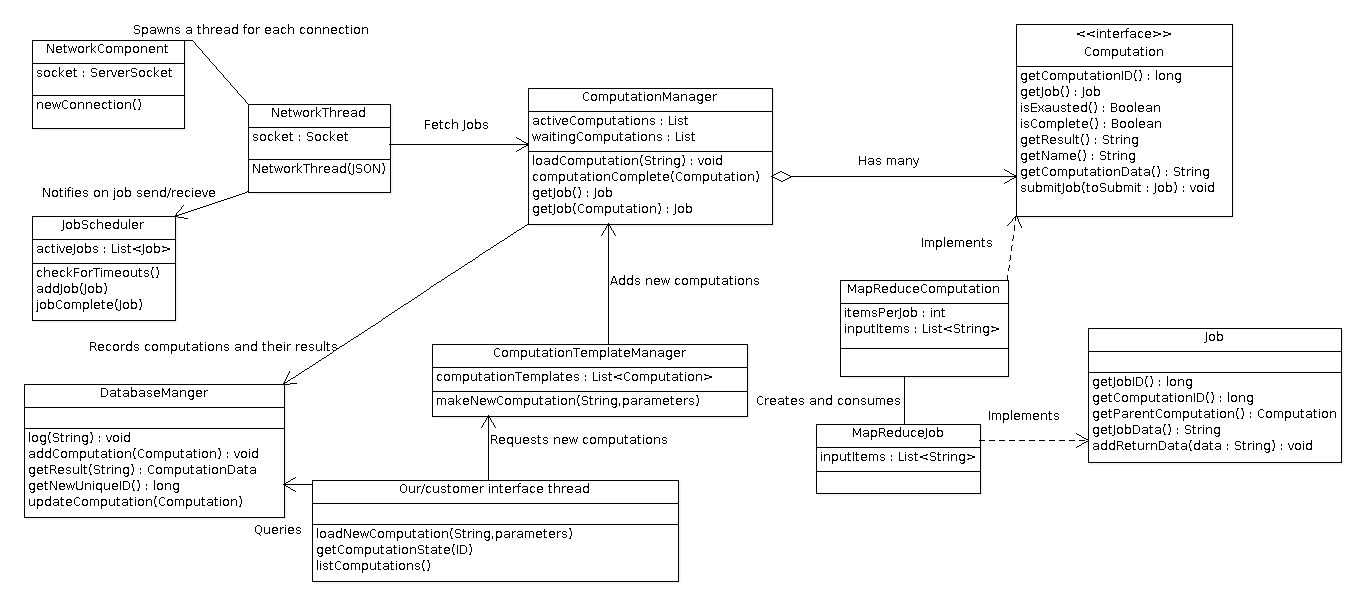
\includegraphics[height=270pt]{serveruml.png}

\subsubsection{Worker Devices}
The app for the worker devices is split into two main functionalities: the Worker App (the user interface) and the Background Service. 

\paragraph{The Worker App:}

The app that provides the user interface. It should include settings that determine when and how computations run, as well as displaying information about them to the user.

\paragraph{The Background Service:} 
Running in the background on the device, this program connects to the main server. Whenever the device is available it will notify the server, sending meta-information (battery life, location, position, charging state) that may aid in tailoring the job to not interfere with the owners' experience. It will receive Jobs from the server as well as the input data for them and send back the result. If the computation fails the device will discard it and resend the job request.



\subsection{Interface Specifications}


\subsubsection{Server to device API}

The device will send requests to which the server will respond.
There will be no ongoing connections, which should reduce load on the server, and minimal state about currently available users, which simplifies the server network component.

\lstinputlisting[language=Ruby]{server_api_json.txt}

\newpage
\subsubsection{Computation interface}

We will extend this interface to create computation templates that the customer provides input for.
\lstinputlisting[language=Java]{../server/Computation.java}
\newpage
\lstinputlisting[language=Java]{../server/ComputationCode.java}

\lstinputlisting[language=Java]{../server/Job.java}

\subsubsection{User interface}
The graphical interface of the user application will enable the user to control various aspects of the computation process, as well as set preferences and constraints. A master toggle can be used to enable or disable the computation service: turning it on will initialise a background service and connect the application to the server. This gives the user a simple way to start and end computations, and also prevents unnecessary processing if the user launches the app accidentally. The user can log in via their Google or Facebook account to access the social features of the application, but this is not necessary. \\
The home screen will give a brief description of the currently running computations, quick settings and short statistics. A navigation menu gives access to the list of computations, detailed statistics, settings and achievements. 
\begin{itemize}
    \item The Computations screen lists the selected computations and lets the user add a new one.
    \item The Statistics screen shows simple graphs and tables that give information about the completed jobs and computations, duration of activity, etc. 
    \item The Achievements screen lists general and computation-specific achievements to provide an incentive for users to use the application.
    \item The Settings screen lets the user tailor the computation process to their needs. Settings include: setting the mobile data usage limit (how much data can be accessed and sent through the mobile network when WiFi is not available – can be 0), battery usage limit (computation should stop when battery level reaches a lower limit), details about location (e.g. computation can be more intensive when phone is at home), scheduling (time periods when computation can become more intensive), notifications, etc.
\end{itemize}
The application also lets the user connect to Facebook and share statistics or achievements which also helps to advertise the application.\par
The computation itself will run in a background service. It will run on the main thread in the background, performing computation while the app is in the background or the phone is sleeping. The computation process can be stopped by turning it off in the app, or closing the app.

\subsubsection{Local database}

A local, shared database will be used to store metadata about the running and completed jobs and computations. The background service adds entries to the database when it receives a new job or computation and after it has finished the process. The user activity (GUI) can then access this database for statistics and evaluating rewards. The underlying implementation will be a local SQLite database.

\begin{multicols}{2}
\paragraph{Computation table:} ~\\
\noindent Name\\
ID\\
Parameters\\
Status: waiting, active, complete, error\\
Result\\
Start time\\
End time

\paragraph{Job table:} ~\\
\noindent Computation ID\\
Job ID\\
Duration\\
Number of bytes sent\\
Number of bytes analysed\\
\end{multicols}


\subsection{Constraints, Assumptions and Dependencies}
\paragraph{Constraints}
\begin{itemize}
	\item The jobs should have small to medium computation in order to make sure at least one job can be solved while, say, the device is charging. This is due to the fact that we don't have direct control of how long the user will let jobs run. This means we can only process computations that can be split into small jobs.

	\item The jobs should restrict the amount of data sent over the network, especially when not using WiFi. This limits the kind of computation we can do.
\end{itemize} 

\paragraph{Assumptions}
\begin{itemize}
	\item We assume the device will allow a service to run at full power while the device sleeps.
	\item We assume that the user will not be using the phone while jobs run.
	\item We assume that the device will protect itself from overheating.
\end{itemize} 

\paragraph{Dependencies}
\begin{itemize}
\item The app depends on the Android SDK and ecosystem.
\item The server will use Java, so depend on OpenJDK and the associated standard library.
\item The app will use SQLite to store settings.
\item The server will use the PostgreSQL database.
\item The server will use Apache HTTP for serving code and large data files.
\item The org.json Java package will be used for JSON parsing.
\end{itemize}

\newpage
\section{Management strategy}

Project manager: Ben Ramchandani

\subsection{Team split by component}

We have split up into smaller sub-groups to work on individual components.
Our management plans are described in the Project Plan document.

\subsubsection{Server}

Ben Ramchandani and Razvan Kusztos.

\subsubsection{App background service}

James Wood and Jack Needham.

\subsubsection{App user interface}

Laura Nechita and Dmitrij Szamozvancev.

\end{document}
